En esta sección se exponen los diversos aspectos relacionados con la planificación del proyecto. Para facilitar la compresión de los datos y figuras que se van a mostrar más adelante, en la tabla \ref{tab:task_id_name}, se expone la relación entre los identificadores de las tareas y sus denominaciones.

\begin{table}[htp]
	\centering
	\caption{Relación identificador-tarea}\label{tab:task_id_name}
	\begin{tabular}{cc}
		\toprule
    	\textbf{Identificador} & \emph{Nombre}\\
    	\midrule
    	T1 & Análisis de herramientas provistas por \acrshort{oai} para implementar el repositorio\\
    	T2 & Análisis de herramientas para desarrollo web\\
    	T3 & Análisis de herramientas semánticas\\
    	T4 & Desarrollo del proveedor\\
    	T5 & Diseño del modelo relacional de datos de \acrshort{oaipmh}\\
    	T6 & Implementación del servidor \acrshort{oaipmh}\\
    	T7 & Desarrollo del front-end del sistema\\
    	T8 & Pruebas del servidor \acrshort{oaipmh}\\
    	T9 & Pruebas de la plataforma web\\
    	T10 & Publicación de la aplicación en el portal web de MORElab\\
    	T11 & Desplegar el servidor \acrshort{oaipmh}\\
    	\bottomrule
    \end{tabular}
\end{table}

\subsection{Diagrama de precedencias}

En esta sección se muestra el diagrama de precedencias (ver figura 2.3).

\begin{figure}[!htbp]
	\centering
	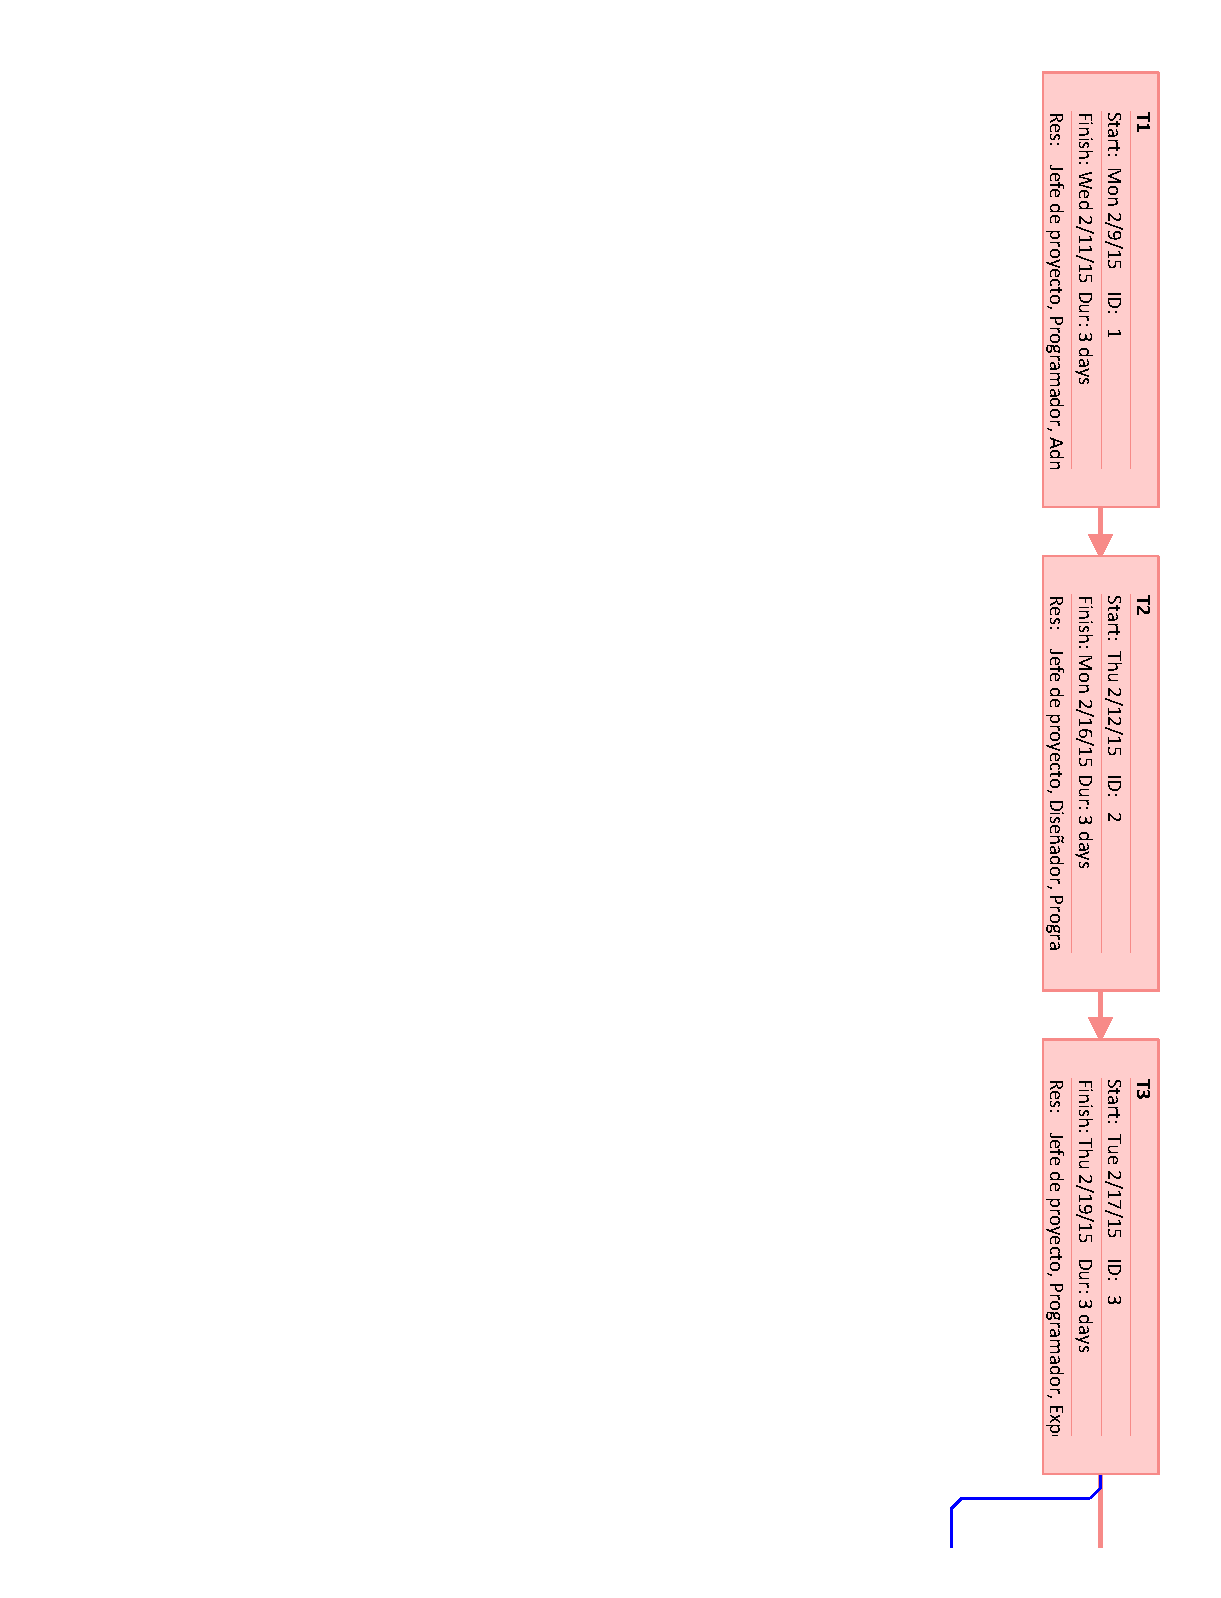
\includegraphics[page=1, scale=.65]{fig/network_diagram}
	\caption{Diagrama de precedencias 1}
\end{figure}

\begin{figure}[!htbp]
	\centering
	\includegraphics[page=2, scale=.65]{fig/network_diagram}
	\caption{Diagrama de precedencias 2}
\end{figure}

\begin{figure}[!htbp]
	\centering
	\includegraphics[page=3, scale=.65]{fig/network_diagram}
	\caption{Diagrama de precedencias 3}
\end{figure}

\begin{figure}[!htbp]
	\centering
	\includegraphics[page=4, scale=.65]{fig/network_diagram}
	\caption{Leyenda del diagrama de precedencias}
\end{figure}